% ======================================================================================================
% NOTES, TODOS
% What is Ditto -> reference the official webisite

% ======================================================================================================

\section{Eclipse Ditto - Digital Twin Setup}
Eclipse Ditto is an open-source framework that provides a way to create and manage Digital Twin of connected devices [ref]. Ditto can be deployed on-premises or in the cloud. For this research, we build and deploy the ditto code base using docker on a virtual private cloud server. 


We have two options for deploying and running Ditto on a cloud Linux server. The first option involves utilizing the Kubernetes cluster, which necessitates substantial infrastructure resources. Specifically, a minimum of 4 GB RAM, 8 core processes, and 20 GB disk storage are required. However, the second option, which we have chosen, involves using Docker. This alternative demands fewer resources compared to the previous one. Under this option, we have seven microservices operating in parallel, each fulfilling distinct functions. These microservices include Nginx as the web server, Ditto Gateway, Ditto Connectivity for managing the device-to-Ditto connectivity, Ditto Thing for overseeing things (representing physical devices), Thing Search for facilitating efficient search using MongoDB, Swagger-UI for providing a web-based user interface, and Ditto Policies for access control on things.

The following steps outline the process required to set up Ditto on a Linux server:

\begin{itemize}
    \item Step 1: Install and configure the Docker demon including the docker composer utility.
    \item Step 2: Clone the Eclipse Ditto code base from the official GitHub page using the command: \texttt{git clone https://github.com/eclipse-ditto/ditto.git}
    \item Start running the Ditto cluster as microservices in a container by executing the command: \texttt{docker-compose up -d}
    \item Verify that all microservices are running and check the health status of Ditto using the following commands: \texttt{curl -u devops:foobar\\ http://localhost:8080/status/health}
\end{itemize}
The process of running Ditto and connecting with the MQTT broker is described below.

\textit{Creating Policy}: In Ditto policies are JSON configuration file that defines who access what. Creating policies is the first step in running Ditto. The policy configuration we use for our project is presented as follows. To speed up experimenting with Ditto we used a bash script that we can run from the terminal of the server. 
\begin{lstlisting}[style=CStyle]
#!/bin/bash

curl -X PUT 'http://localhost:8080/api/2/policies/ut.thesis.demo:policy' -u 'ditto:ditto' -H 'Content-Type: application/json' -d '{
    "entries": {
        "owner": {
            "subjects": {
                "nginx:ditto": {
                    "type": "nginx basic auth user"
                }
            },
            "resources": {
                "thing:/": {
                    "grant": [
                        "READ","WRITE"
                    ],
                    "revoke": []
                },
                "policy:/": {
                    "grant": [
                        "READ","WRITE"
                    ],
                    "revoke": []
                },
                "message:/": {
                    "grant": [
                        "READ","WRITE"
                    ],
                    "revoke": []
                }
            }
        }
    }
}'

\end{lstlisting}

\textit{Creating things}: Things are the digital representation of the physical device with attributes and features. Like we did for policy, for the thing we also created bash script as follow. 

\begin{lstlisting}[style=CStyle]
    

#!/bin/bash

curl -X PUT 'http://localhost:8080/api/2/things/ut-sensors:esp01' -u 'ditto:ditto' -H 'Content-Type: application/json' -d '{
    "policyId": "ut.thesis.demo:policy",
    "attributes": {
        "name": "Esp3201",
        "type": "Esp32 board"
    },
    "features": {
        "temperature": {
            "properties": {
                "value": 0
            }
        },
        "altitude": {
            "properties": {
                "value": 0
            }
        }
    }
}'
\end{lstlisting}

\textit{Creating connection:} The connection configuration file serves the purpose of defining the source and target of the MQTT broker topic. In this case, the connection type is MQTT, and the specified URI contains the IP address. The source topic is set as "ut-sensors/\#", indicating that Ditto will receive data from the broker when a message is published on any topic under "ut-sensors". On the other hand, the target address is defined as "ut-sensors/{{thing:id}}", which means that Ditto will publish data on the corresponding topic of the device whenever an event is emitted by the thing with the given ID. The inclusion of "\#" at the end of the string signifies that messages can be received from any topic under "ut-sensors". This configuration enables bidirectional communication and data exchange between Ditto and IoT devices via the MQTT broker. 

\begin{lstlisting}[style=CStyle]
#!/bin/bash

curl -X POST 'http://localhost:8080/devops/piggyback/connectivity?timeout=10' -u 'devops:foobar' -H 'Content-Type: application/json' -d '{
    "targetActorSelection": "/system/sharding/connection",
    "headers": {
        "aggregate": false
    },
    "piggybackCommand": {
        "type": "connectivity.commands:createConnection",
        "connection": {
            "id": "ascon-ut-mqtt-connection",
            "connectionType": "mqtt",
            "connectionStatus": "open",
            "failoverEnabled": true,
            "uri": "tcp://<IP address>:1883",
            "sources": [{
                "addresses": ["ut-sensors/#"],
                "authorizationContext": ["nginx:ditto"],
                "qos": 0,
                "filters": [],
                                "headerMapping": {},
                                "payloadMapping": ["AsconPayload"],
                                "replyTarget": {
                                        "headerMapping": {},
                                        "expectedResponseTypes": [
                                          "response",
                                          "error"
                                        ],
                                        "enabled":false
                                }
            }],
                        "targets": [{
                                "address": "ut-sensors/{{ thing:id }}",
                                "topics": [
                                "_/_/things/twin/events",
                                "_/_/things/live/messages"
                                ],
                                "authorizationContext": ["nginx:ditto"],
                                "headerMapping": {},
                "qos": 0,
                "payloadMapping": ["AsconPayload"]
                        }]
        }
    }
}'
\end{lstlisting}


The other important component of Ditto that works hand in hand is MQTT broker. In the following section we provide detail of how setup it and start running. 

Another crucial component that works hand in hand with Ditto is the MQTT broker. In the subsequent section, we will deep dive into the detailed process of setting it up and initiating its operation.

\section{Building MQTT Broker (Mosquitto) from Source}

The MQTT broker is a lightweight protocol designed for IoT communication[ref]. In our project, we utilized the MQTT implementation from Eclipse Ditto, specifically Mosquitto. To ensure full control and customization, we built the MQTT implementation from the source on our Linux server. This approach was undertaken primarily to accommodate the implementation of the lightweight encryption algorithm into the source code. However, we later decided to implement the algorithms by extending the ditto source code itself through the connectivity extension provided. 

In order to run the MQTT broker on our Linux server, there are a few necessary steps to follow. Firstly, we need to install a couple of dependencies, namely \texttt{libcjson-dev and libwebsocket-dev}. Once these dependencies are installed, we proceed to build the source code by executing the following command: \texttt{make WITH\_SRV=yes WITH\_TLS=no WITH\_WEBSOCKETS=yes WITH\_CJSON = yes WITH\_BUNDLED\_DEPS = yes WITH\_DOCS=no}. After the build process, we can verify the successful installation of MQTT by running the tests using the command \texttt{make test}. Finally, to complete the installation, we execute \texttt{sudo make install} to install the MQTT broker into our system. 


It is worth noting that the MQTT broker can be installed either on the same machine as the Ditto running machine or on a different remotely accessible machine. Our proposed scheme ensures secure communication between the IoT device and the cloud-hosted Ditto service. The MQTT broker has limited visibility, as it can only access the encrypted payload, thereby preventing any malicious broker from compromising the security of the communication. The lightweight authentication and encryption algorithm we leverage into our proposed solution guarantees the confidentiality and integrity of the data exchanged.

To start the MQTT service, there are two options available. The first option is to execute the command "mosquitto" directly. Alternatively, we can start the MQTT service with additional configuration options by specifying the configuration file path using the following command: "mosquitto -v -c /path/to/mosquitto.conf".

To publish and subscribe to topics using the MQTT broker, we utilize the commands provided on the GitHub page of Mosquitto. 
    \begin{itemize}
        \item For subscribing to a topic, we employ the command "mosquitto\_sub -t 'test/topic' -v". This command enables us to subscribe to the specified topic and receive the messages associated with it. 
        \item To publish a message to a topic, we run "mosquitto\_pub -t 'test/topic' -m 'hello world'". By executing this command, we can publish a message to the specified topic so that other subscribers to the topic get notified. 
    \end{itemize}
    
    
% \begin{figure}[H]
%     \caption{Ditto Architecture}
%     \centering
%     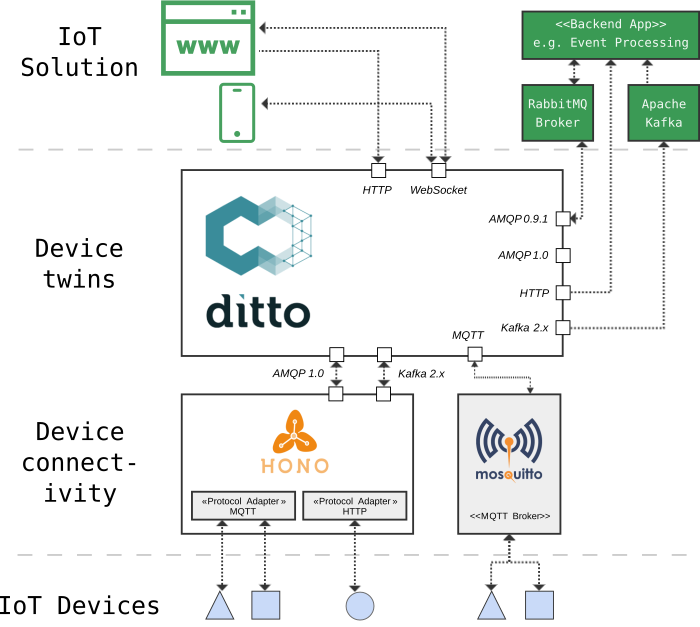
\includegraphics[width=\textwidth]{images/fp/ditto-overview-1.png}
%     \label{fig:ditto-arch}
% \end{figure}
